\documentclass{article}
\usepackage{amsmath}
\usepackage{amssymb}
\usepackage{amsbsy}
\usepackage{bbm}
\usepackage{url}
\usepackage{color}
\usepackage{float}
\usepackage{graphicx}
\usepackage{epstopdf}
\usepackage{fancyhdr}
\usepackage{enumerate}
\usepackage{tikz}
\usepackage[ruled,vlined]{algorithm2e}
\usepackage[colorlinks=true,urlcolor=blue]{hyperref}
\usepackage[utf8]{inputenc}
\numberwithin{figure}{section}

\newcommand{\Solution}[1]{%
    {%
        \medskip
        \color{red}
        \bf $\bigstar$~\sf\textbf{Solution}~$\bigstar$ \sf
        #1
    }
    \bigskip
}


\graphicspath{{assets}{Homework 2/assets/}}

\title{CS224W Homework 2}
\date{Due: November 4, 2024}

\begin{document}

\maketitle

% Last used - Aut2425
\section{Node Embeddings with TransE [21 points]}

While many real world systems are effectively modeled as graphs, graphs can be a cumbersome format for certain downstream applications, such as machine learning models. It is often useful to represent each node of a graph as a vector in a continuous low dimensional space. The goal is to preserve information about the structure of the graph in the vectors assigned to each node. For instance, the spectral embedding preserved structure in the sense that nodes connected by an edge were usually close together in the (one-dimensional) embedding $x$.\\

\noindent Multi-relational graphs are graphs with multiple types of edges. They are incredibly useful for representing structured information, as in knowledge graphs. There may be one node representing “Washington, DC” and another representing “United States”, and an edge between them with the type “Is capital of”. In order to create an embedding for this type of graph, we need to capture information about not just which edges exist, but what the types of those edges are. In this problem, we will explore a particular algorithm designed to learn node embeddings for multi-relational graphs. \\\\
The algorithm we will look at is TransE.\footnote{See the 2013 NeurIPS paper by Bordes et al: \url{https://papers.nips.cc/paper/5071-translating-embeddings-for modeling-multi-relational-data.pdf}}
We will first introduce some notation used in the paper describing this algorithm.
We’ll let a multi-relational graph $G = (E, S, L)$ consist of the set of \textit{entities} $E$ (i.e., nodes), a set of edges $S$, and a set of possible relationships $L$.
The set $S$ consists of triples $(h, l, t)$, where $h \in E$ is the \textit{head} or source-node, $l \in L$ is the relationship, and $t \in E$ is the \textit{tail} or destination-node.
As a node embedding, TransE tries to learn embeddings of each entity $e \in E$ into $\mathbb{R}^k$ ( $k$-dimensional vectors), which we will notate by $\mathbf{e}$. The main innovation of TransE is that each relationship $\ell$ is also embedded as a vector $\ell \in \mathbb{R}^k$, such that the difference between the embeddings of entities linked via the relationship $\ell$ is approximately $\ell$. That is, if $(h, \ell, t) \in S$, TransE tries to ensure that $\mathbf{h}+\boldsymbol{\ell} \approx \mathbf{t}$. Simultanesouly, TransE tries to make sure that $\mathbf{h}+\boldsymbol{\ell} \not\approx \mathbf{t}$ if the edge $(h, \ell, t)$ does not exist.\\\\
\textbf{Note on notation}: we will use unbolded letters $e, \ell$, etc. to denote the entities and relationships in the graph, and bold letters $\mathbf{e}, \boldsymbol{\ell}$, etc., to denote their corresponding embeddings.
TransE accomplishes this by minimizing the following loss:
\begin{equation}\label{eq1}
\mathcal{L}=\sum_{(h, \ell, t) \in S}\left(\sum_{\left(h^{\prime}, \ell, t^{\prime}\right) \in S_{(h, \ell, t)}^{\prime}}\left[\gamma+d(\mathbf{h}+\boldsymbol{\ell}, \mathbf{t})-d\left(\mathbf{h}^{\prime}+\boldsymbol{\ell}, \mathbf{t}^{\prime}\right)\right]_{+}\right)
\end{equation}
Here $\left(h^{\prime}, \ell, t^{\prime}\right)$ are "corrupted" triplets, chosen from the set $S_{(h, \ell, t)}^{\prime}$ of corruptions of $(h, \ell, t)$, which are all triples where either $h$ or $t$ (but not both) is replaced by a random entity, and $\ell$ remains the same as the one in the original triplets.
$$
S_{(h, \ell, t)}^{\prime}=\left\{\left(h^{\prime}, \ell, t\right) \mid h^{\prime} \in E\right\} \cup\left\{\left(h, \ell, t^{\prime}\right) \mid t^{\prime} \in E\right\}
$$
Additionally, $\gamma>0$ is a fixed scalar called the \textit{margin}, the function $d(\cdot, \cdot)$ is the Euclidean distance, and $[\cdot]_{+}$ is the positive part function (defined as $\max (0, \cdot)$). Finally, TransE restricts \textbf{all the entity embeddings to have length $1:\|\mathbf{e}\|_2=1$ for every $e \in E$.}\\
For reference, here is the TransE algorithm, as described in the original paper on page 3:
\begin{figure}[H]
    \centering
    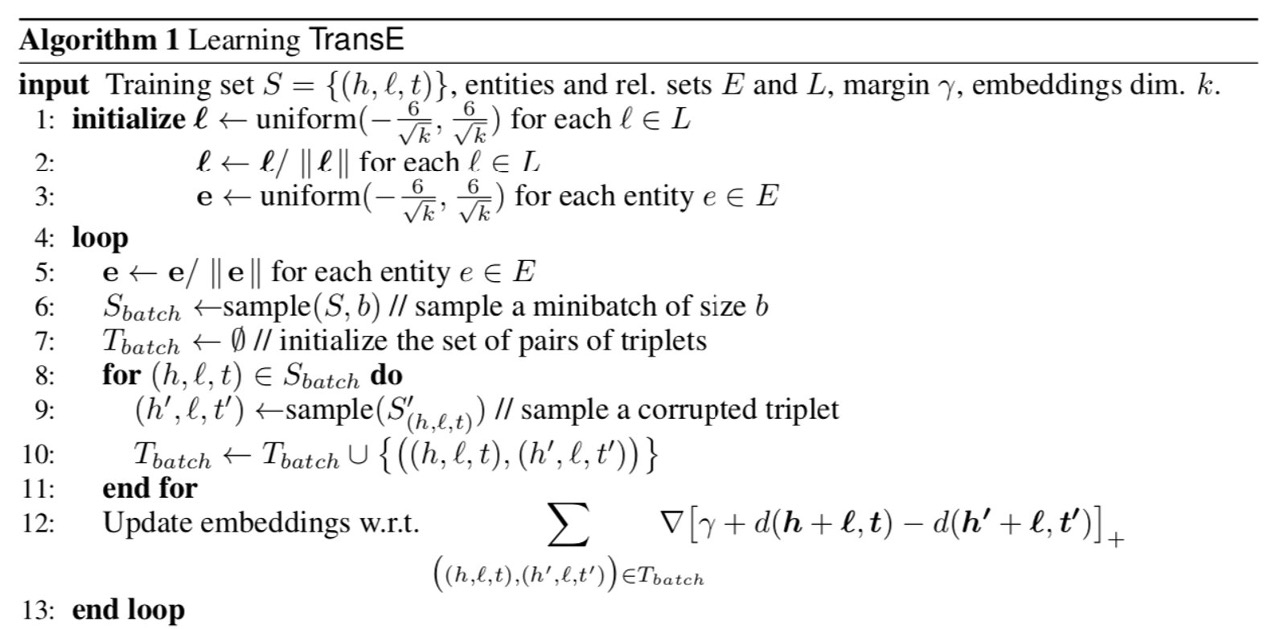
\includegraphics[width=1.0\textwidth]{algo2.png}
    \label{fig:algo2}
\end{figure}

\subsection{Simplified Objective [3 points]}
Say we were intent on using a simpler loss function. Our objective function (\ref{eq1}) includes a term maximizing the distance between $\mathbf{h}^{\prime}+\boldsymbol{\ell}$ and $\mathbf{t}^{\prime}$. If we instead simplified the objective, and just tried to minimize
\begin{equation}\label{eq2}
\mathcal{L}_{\text {simple }}=\sum_{(h, \ell, t) \in S} d(\mathbf{h}+\boldsymbol{\ell}, \mathbf{t}),
\end{equation}

we would obtain a useless embedding. Give an example of a simple graph and corresponding embeddings which will minimize the new objective function (\ref{eq2}) all the way to zero, but still give a completely useless embedding.\\
\textbf{Hint:} Your graph should be non-trivial, i.e., it should include at least two nodes and at least one edge. Assume the embeddings are in 2 dimensions, i.e., $k = 2$.
What happens if $\boldsymbol{\ell} = \textbf{0}$?

\Solution{
	A useless embedding can be achieved by setting all entity embeddings to be identical and all relation embeddings to be the zero vector.
	
	\textbf{Example Graph and Embeddings:}
	\begin{itemize}
		\item \textbf{Graph:} Consider a simple graph with two entities, $A$ and $B$, and one relationship type, $R$. The graph contains a single edge $(A, R, B)$.
		\item \textbf{Embeddings:} Let the embeddings be in 2D space ($k=2$). We can set the embeddings as follows:
		\begin{itemize}
			\item $\mathbf{a} = [0.5, 0.5]$
			\item $\mathbf{b} = [0.5, 0.5]$
			\item $\boldsymbol{\ell_R} = [0, 0]$
		\end{itemize}
	\end{itemize}
	
	\textbf{Minimizing the Objective to Zero:}
	With these embeddings, the objective function becomes:
	\[ \mathcal{L}_{\text {simple }} = d(\mathbf{a} + \boldsymbol{\ell_R}, \mathbf{b}) = \left\| (\mathbf{a} + \boldsymbol{\ell_R}) - \mathbf{b} \right\|_2 \]
	\[ = \left\| ([0.5, 0.5] + [0, 0]) - [0.5, 0.5] \right\|_2 = \left\| [0.5, 0.5] - [0.5, 0.5] \right\|_2 = \left\| [0, 0] \right\|_2 = 0 \]
	The objective is minimized perfectly to zero.
	
	\textbf{Why the Embedding is Useless:}
	This embedding is useless because every entity in the graph is mapped to the exact same point in the embedding space. The model has learned no distinguishing features between the nodes. It is impossible to use these embeddings to determine if two nodes are the same or different, let alone predict relationships between them.
}

\subsection{Utility of $\gamma$  [5 points]}
We are interested in understanding what the margin term $\gamma$ accomplishes. If we removed the margin term $\gamma$ from our loss, and instead optimized
\begin{equation}\label{eq3}
\mathcal{L}_{\text {no margin }}=\sum_{(h, \ell, t) \in S} \sum_{\left(h^{\prime}, \ell t^{\prime}\right) \in S_{(h, \ell, t)}^{\prime}}\left[d(\mathbf{h}+\boldsymbol{\ell}, \mathbf{t})-d\left(\mathbf{h}^{\prime}+\boldsymbol{\ell}, \mathbf{t}^{\prime}\right)\right]_{+},
\end{equation}
it turns out that we would again obtain a useless embedding. Give an example of a simple graph and corresponding embeddings which will minimize the new objective function (\ref{eq3}) all the way to zero, but still give a completely useless embedding. By useless, we mean that in your example, you cannot tell just from the embeddings whether two nodes are linked by a particular relation (Note: your graph should be non-trivial, i.e., it should include at least two nodes and at least one edge. Assume the embeddings are in 2 dimensions, i.e., $k=2$.)

\Solution{
	A useless embedding can be achieved by collapsing all entities and relations into a state where the distance for any true triplet is equal to the distance for any corrupted triplet. The simplest way to achieve this is to make all these distances zero.
	
	\textbf{Example Graph and Embeddings:}
	\begin{itemize}
		\item \textbf{Graph:} Consider a graph with two entities, $A$ and $B$, and one relationship $R$, forming the edge $(A, R, B)$.
		\item \textbf{Embeddings:} Let all entity embeddings be identical, and the relation embedding be the zero vector.
		\begin{itemize}
			\item $\mathbf{a} = [0.5, 0.5]$
			\item $\mathbf{b} = [0.5, 0.5]$
			\item $\boldsymbol{\ell_R} = [0, 0]$
		\end{itemize}
	\end{itemize}
	
	\textbf{Minimizing the Objective to Zero:}
	The loss for the true triplet $(A, R, B)$ is a sum over all its "corrupted" versions. Let's consider any corrupted triplet, for example $(A', R, B)$ where $A'$ is another entity in the graph. Since all entity embeddings are identical, $\mathbf{a'} = \mathbf{a} = \mathbf{b} = [0.5, 0.5]$.
	
	We calculate the distance for the true triplet, $d_{\text{pos}}$, and the corrupted triplet, $d_{\text{neg}}$:
	\begin{itemize}
		\item $d_{\text{pos}} = d(\mathbf{a} + \boldsymbol{\ell_R}, \mathbf{b}) = \left\| ([0.5, 0.5] + [0, 0]) - [0.5, 0.5] \right\|_2 = 0$.
		\item $d_{\text{neg}} = d(\mathbf{a'} + \boldsymbol{\ell_R}, \mathbf{b}) = \left\| ([0.5, 0.5] + [0, 0]) - [0.5, 0.5] \right\|_2 = 0$.
	\end{itemize}
	
	The contribution to the loss for this specific corruption is:
	\[ [d_{\text{pos}} - d_{\text{neg}}]_+ = [0 - 0]_+ = 0 \]
	Since this holds for any possible corruption (as all entity embeddings are the same), the total loss $\mathcal{L}_{\text{no margin}}$ is zero.
	
	\textbf{Why the Embedding is Useless:}
	This embedding is useless for the same reason as in the previous question: all entities are mapped to a single point, making them indistinguishable. The model has perfectly minimized the loss without learning any of the graph's structure. The margin term $\gamma$ is crucial because it prevents this collapse by forcing a separation ($d_{\text{pos}} + \gamma \leq d_{\text{neg}}$), which cannot be satisfied when both distances are zero.
}

\subsection{ Normalizing the embeddings [5 points]}
Recall that TransE normalizes every entity embedding to have unit length (see line 5 of the algorithm). The quality of our embeddings would be much worse if we did not have this step. To understand why, imagine running the algorithm with line 5 omitted.
What could the algorithm do to trivially minimize the loss in this case? What would the embeddings
it generates look like?

\Solution{
	If the normalization step (line 5 of the algorithm) were omitted, the model could trivially minimize the loss function by driving the norms of the entity embeddings to infinity.
	
	\textbf{Trivial Minimization Strategy:}
	The objective is to satisfy the inequality $d(\mathbf{h}+\boldsymbol{\ell}, \mathbf{t}) + \gamma \leq d(\mathbf{h'}+\boldsymbol{\ell}, \mathbf{t'})$ for all true triplets $(h, \ell, t)$ and their corrupted versions. This is equivalent to $\|\mathbf{h}+\boldsymbol{\ell}-\mathbf{t}\|_2 + \gamma \leq \|\mathbf{h'}+\boldsymbol{\ell}-\mathbf{t'}\|_2$.
	
	Without the normalization constraint, the algorithm can learn embeddings with arbitrarily large magnitudes. The model can simply scale up the norms of all entity embeddings by a very large factor $M \rightarrow \infty$.
	Let the scaled embeddings be $\mathbf{e}_{\text{new}} = M \cdot \mathbf{e}$ for every entity $e \in E$. The inequality becomes:
	\[ \|M\mathbf{h}+\boldsymbol{\ell}-M\mathbf{t}\|_2 + \gamma \leq \|M\mathbf{h'}+\boldsymbol{\ell}-M\mathbf{t'}\|_2 \]
	As $M$ becomes very large, the contribution of the relation vector $\boldsymbol{\ell}$ becomes negligible compared to the entity embeddings. The inequality approaches:
	\[ M\|\mathbf{h}-\mathbf{t}\|_2 + \gamma \leq M\|\mathbf{h'}-\mathbf{t'}\|_2 \]
	Dividing by $M$, we get:
	\[ \|\mathbf{h}-\mathbf{t}\|_2 + \frac{\gamma}{M} \leq \|\mathbf{h'}-\mathbf{t'}\|_2 \]
	As $M \rightarrow \infty$, the term $\frac{\gamma}{M} \rightarrow 0$. The model now only needs to satisfy $\|\mathbf{h}-\mathbf{t}\|_2 \leq \|\mathbf{h'}-\mathbf{t'}\|_2$, which it can achieve with minimal learning. The loss can be made arbitrarily close to zero by simply increasing the magnitude of all entity embeddings indefinitely.
	
	\textbf{Resulting Embeddings:}
	The embeddings generated would be useless. Their magnitudes would grow without bound during training, leading to numerical instability. The final embeddings would have enormous norm values, and the meaningful geometric relationships that TransE is designed to capture would be lost. The normalization step is crucial as it constrains the embeddings to a compact space (the surface of a unit hypersphere), forcing the model to learn meaningful angular and directional relationships rather than simply scaling magnitudes.
}

\subsection{Expressiveness of TransE embeddings [8 points]}
Give an example of a simple graph for which no perfect embedding exists, i.e., no embedding perfectly satisfies $\mathbf{u}+\boldsymbol{\ell}=\mathbf{v}$ for all $(u, \ell, v) \in S$ and $\mathbf{u}+\boldsymbol{\ell} \neq \mathbf{v}$ for $(u, \ell, v) \notin S$, for any choice of entity embeddings ($\mathbf{e}$ for $e \in E$ ) and relationship embeddings ( $\boldsymbol{\ell}$ for $\ell \in L$ ). Explain why this graph has no perfect embedding in this system, and what that means about the expressiveness of TransE embeddings. As before, assume the embeddings are in 2 dimensions $(k=2)$.\\
\textbf{Hint: }By expressiveness of TransE embeddings, we want you to talk about which type of relationships TransE can/cannot model with an example. (Note that the condition for this question is slightly different from that for Question 2.1 and what we ask you to answer is different as well).

\Solution{
	\textbf{Example Graph:}
	A simple graph for which no perfect TransE embedding exists is one that models a symmetric relationship. Consider a graph with two entities, $A$ and $B$, and a single symmetric relationship type, $R$ (e.g., "is friends with"). The set of edges $S$ contains two triplets:
	\[ S = \{ (A, R, B), (B, R, A) \} \]
	Let's also assume there is another entity $C$ not related to $A$ or $B$, so $(A, R, C) \notin S$.
	
	\textbf{Why No Perfect Embedding Exists:}
	A perfect embedding must satisfy $\mathbf{h}+\boldsymbol{\ell} = \mathbf{t}$ for all true triplets and $\mathbf{h}+\boldsymbol{\ell} \neq \mathbf{t}$ for all false triplets.
	
	\begin{enumerate}
		\item From the triplet $(A, R, B)$, a perfect embedding requires:
		\[ \mathbf{a} + \boldsymbol{\ell_R} = \mathbf{b} \quad \implies \quad \boldsymbol{\ell_R} = \mathbf{b} - \mathbf{a} \]
		\item From the triplet $(B, R, A)$, a perfect embedding requires:
		\[ \mathbf{b} + \boldsymbol{\ell_R} = \mathbf{a} \quad \implies \quad \boldsymbol{\ell_R} = \mathbf{a} - \mathbf{b} \]
	\end{enumerate}
	
	Combining these two requirements, we get $\mathbf{b} - \mathbf{a} = \mathbf{a} - \mathbf{b}$, which simplifies to $2\mathbf{b} = 2\mathbf{a}$, or $\mathbf{a} = \mathbf{b}$. This means that for TransE to perfectly model this relationship, the embeddings for entities $A$ and $B$ must be identical.
	
	Furthermore, if we substitute $\mathbf{a} = \mathbf{b}$ back into the first equation, we get $\boldsymbol{\ell_R} = \mathbf{a} - \mathbf{a} = \mathbf{0}$. So, the relation embedding must be the zero vector.
	
	This leads to a contradiction. If $\mathbf{a} = \mathbf{b}$ and $\boldsymbol{\ell_R} = \mathbf{0}$, then for the false triplet $(A, R, C)$, the model would check if $\mathbf{a} + \boldsymbol{\ell_R} \neq \mathbf{c}$, which is $\mathbf{a} \neq \mathbf{c}$. This part is fine. However, the model has completely lost the ability to distinguish between $A$ and $B$, which is a failure. The very purpose of an embedding is to provide a unique representation for each entity. By forcing $\mathbf{a} = \mathbf{b}$, the model has failed.
	
	\textbf{Expressiveness of TransE Embeddings:}
	This example demonstrates a key limitation in the expressiveness of TransE. The translational model ($ \mathbf{h}+\boldsymbol{\ell} \approx \mathbf{t}$) is inherently directional and struggles to capture relationships that are not one-to-one or one-to-many. Specifically, \textbf{TransE cannot effectively model symmetric (or many-to-many) relations}. It is forced to learn identical embeddings for entities linked by such relations and a zero vector for the relation itself, which is not a useful representation. TransE's expressiveness is thus best suited for hierarchical or directed, non-symmetric relationships.
}
% \textbf{What to Submit}
% \begin{enumerate}
%     \item Graph and corresponding useless embeddings which minimize (\ref{eq2}) to 0.
%     \item Graph and corresponding useless embeddings which minimize (\ref{eq3}) to 0 .
%     \item Discussion of behavior of algorithm and resulting embeddings without normalization step.
%     \item 
%     \begin{itemize}
%         \item Graph for which no perfect embedding exists, with justification.
%         \item Discussion on TransE embedding expressiveness.
%     \end{itemize}
% \end{enumerate}




% Last used - Aut2425
\section{Expressive Power of Knowledge Graph Embeddings [10 points]}
TransE is a common method for learning representations of entities and relations in a knowledge graph. Given a triplet $(h, \ell, t)$, where entities embedded as $h$ and $t$ are related by a relation embedded as $\ell$, TransE trains entity and relation embeddings to make $h+\ell$ close to $t$. There are some common patterns that relations form:
\begin{itemize}
    \item Symmetry: A is married to B, and B is married to A.
    \item Inverse: A is teacher of B, and B is student of A. Note that teacher and student are 2 different relations and have their own embeddings.
    \item Composition: $\mathrm{A}$ is son of $\mathrm{B} ; \mathrm{C}$ is sister of $\mathrm{B}$, then $\mathrm{C}$ is aunt of $\mathrm{A}$. Again note that son, sister, and aunt are 3 different relations and have their own embeddings.
\end{itemize}
\subsection{TransE Modeling [3 points]}
For each of the above relational patterns, can TransE model it perfectly, such that $h+\ell=t$ for all relations? Explain why or why not. Note that here $\mathbf{0}$ embeddings for relation are undesirable since that means two entities related by that relation are identical and not distinguishable.

\Solution{
	\begin{itemize}
		\item \textbf{Symmetry: No.}
		
		A symmetric relation `l` between entities `h` and `t` implies two facts: $(h, l, t)$ and $(t, l, h)$. For TransE to model this perfectly, both equations must hold:
		\begin{enumerate}
			\item $\mathbf{h} + \boldsymbol{\ell} = \mathbf{t}$
			\item $\mathbf{t} + \boldsymbol{\ell} = \mathbf{h}$
		\end{enumerate}
		Substituting the first equation into the second gives $(\mathbf{h} + \boldsymbol{\ell}) + \boldsymbol{\ell} = \mathbf{h}$, which simplifies to $2\boldsymbol{\ell} = \mathbf{0}$, meaning $\boldsymbol{\ell} = \mathbf{0}$. This is an undesirable trivial solution, as it implies the two related entities are identical ($\mathbf{h} = \mathbf{t}$). Therefore, TransE cannot model symmetric relations non-trivially.
		
		\item \textbf{Inverse: Yes.}
		
		An inverse relation pattern involves two different relations, $\ell_1$ and $\ell_2$, such that $(h, \ell_1, t)$ implies $(t, \ell_2, h)$. The two equations are:
		\begin{enumerate}
			\item $\mathbf{h} + \boldsymbol{\ell_1} = \mathbf{t}$
			\item $\mathbf{t} + \boldsymbol{\ell_2} = \mathbf{h}$
		\end{enumerate}
		From the first equation, we have $\boldsymbol{\ell_1} = \mathbf{t} - \mathbf{h}$. From the second, we have $\boldsymbol{\ell_2} = \mathbf{h} - \mathbf{t}$. This leads to the consistent and non-trivial solution $\boldsymbol{\ell_2} = - \boldsymbol{\ell_1}$. TransE can model inverse relations perfectly by learning relation vectors that are negatives of each other.
		
		\item \textbf{Composition: Yes.}
		
		A composition pattern involves three relations, $\ell_1, \ell_2, \ell_3$, such that $(h, \ell_1, z)$ and $(z, \ell_2, t)$ implies $(h, \ell_3, t)$. The three equations are:
		\begin{enumerate}
			\item $\mathbf{h} + \boldsymbol{\ell_1} = \mathbf{z}$
			\item $\mathbf{z} + \boldsymbol{\ell_2} = \mathbf{t}$
			\item $\mathbf{h} + \boldsymbol{\ell_3} = \mathbf{t}$
		\end{enumerate}
		By substituting the first equation into the second, we get $(\mathbf{h} + \boldsymbol{\ell_1}) + \boldsymbol{\ell_2} = \mathbf{t}$. Comparing this with the third equation, we must have $\mathbf{h} + \boldsymbol{\ell_1} + \boldsymbol{\ell_2} = \mathbf{h} + \boldsymbol{\ell_3}$, which simplifies to $\boldsymbol{\ell_3} = \boldsymbol{\ell_1} + \boldsymbol{\ell_2}$. This is a valid, non-trivial solution where the composed relation vector is the sum of the component relation vectors. TransE can model composition perfectly.
	\end{itemize}
}

\subsection{RotatE Modeling [3 points]}
Consider a new model, RotatE. Instead of training embeddings such that $h+\ell \approx t$, we train embeddings such that $h \circ \ell \approx t$. Here $\circ$ means rotation. You can think of $h$ as a vector of dimension $2 d$, representing $d$ $2 \mathrm{D}$ points. $\ell$ is a $d$-dimensional vector specifying rotation angles. When applying $\circ$, For all $i \in 0 \ldots d-1, \left(h_{2 i}, h_{2 i+1}\right)$ is rotated clockwise by $l_i$. Similar to TransE, the entity embeddings are also normalized to L2 norm 1. Can RotatE model the above 3 relation patterns perfectly? Why or why not?

\Solution{
	In RotatE, the model aims to satisfy $\mathbf{h} \circ \boldsymbol{\ell} = \mathbf{t}$, where embeddings are in the complex plane and $\circ$ represents complex multiplication. We also have $|\mathbf{h}|=1$ for all entities $h$. For a relation $\ell$ to be a pure rotation, we must have $|\boldsymbol{\ell}|=1$.
	
	\begin{itemize}
		\item \textbf{Symmetry: Yes.}
		
		A symmetric relation $\ell$ implies $\mathbf{h} \circ \boldsymbol{\ell} = \mathbf{t}$ and $\mathbf{t} \circ \boldsymbol{\ell} = \mathbf{h}$.
		Substituting the first equation into the second gives $(\mathbf{h} \circ \boldsymbol{\ell}) \circ \boldsymbol{\ell} = \mathbf{h}$, which means $\mathbf{h} \circ \boldsymbol{\ell}^2 = \mathbf{h}$.
		This simplifies to $\boldsymbol{\ell}^2 = 1$. In the complex plane, this has two solutions: $\boldsymbol{\ell} = 1$ (0-degree rotation) or $\boldsymbol{\ell} = -1$ (180-degree rotation). The $\boldsymbol{\ell}=-1$ solution is non-trivial and perfectly models symmetry: applying a 180-degree rotation twice returns the original vector.
		
		\item \textbf{Inverse: Yes.}
		
		An inverse relation pattern involves two relations, $\ell_1$ and $\ell_2$, such that $\mathbf{h} \circ \boldsymbol{\ell_1} = \mathbf{t}$ and $\mathbf{t} \circ \boldsymbol{\ell_2} = \mathbf{h}$.
		From the first equation, we get $\mathbf{h} = \mathbf{t} / \boldsymbol{\ell_1}$. From the second, we get $\mathbf{t} = \mathbf{h} / \boldsymbol{\ell_2}$.
		This leads to the consistent, non-trivial solution where $\boldsymbol{\ell_2} = 1 / \boldsymbol{\ell_1} = \boldsymbol{\ell_1}^{-1}$. This means the second relation is the inverse rotation of the first (e.g., if one is a +45 degree rotation, the other is a -45 degree rotation). RotatE can model this perfectly.
		
		\item \textbf{Composition: Yes.}
		
		A composition pattern involves three relations, $\ell_1, \ell_2, \ell_3$, such that $\mathbf{h} \circ \boldsymbol{\ell_1} = \mathbf{z}$ and $\mathbf{z} \circ \boldsymbol{\ell_2} = \mathbf{t}$ implies $\mathbf{h} \circ \boldsymbol{\ell_3} = \mathbf{t}$.
		Substituting the first equation into the second gives $(\mathbf{h} \circ \boldsymbol{\ell_1}) \circ \boldsymbol{\ell_2} = \mathbf{t}$, which simplifies to $\mathbf{h} \circ (\boldsymbol{\ell_1} \circ \boldsymbol{\ell_2}) = \mathbf{t}$.
		Comparing this with the third equation, $\mathbf{h} \circ \boldsymbol{\ell_3} = \mathbf{t}$, we get the non-trivial solution $\boldsymbol{\ell_3} = \boldsymbol{\ell_1} \circ \boldsymbol{\ell_2}$. The composed relation corresponds to the product of the component relation rotations. RotatE can model this perfectly.
	\end{itemize}
}

\subsection{Failure Cases [4 points]}
Give an example of a graph that RotatE cannot model. Can TransE model this graph? Assume that relation embeddings cannot be $\mathbf{0}$ in either model.

\Solution{
	\textbf{Example Graph:}
	Consider a simple graph representing a symmetric relationship, which RotatE can model but TransE cannot (given the constraints).
	Let the graph contain two entities, A and B, and one relation R (e.g., "is\_roommate\_with"). The graph consists of two facts:
	\begin{itemize}
		\item $(A, R, B)$
		\item $(B, R, A)$
	\end{itemize}
	
	\textbf{Why RotatE Can Model This Graph:}
	RotatE needs to satisfy two equations:
	\begin{enumerate}
		\item $\mathbf{a} \circ \boldsymbol{\ell_R} = \mathbf{b}$
		\item $\mathbf{b} \circ \boldsymbol{\ell_R} = \mathbf{a}$
	\end{enumerate}
	As shown in question 2.2, this is perfectly modeled by setting the relation $\boldsymbol{\ell_R}$ to be a 180-degree rotation (i.e., $\boldsymbol{\ell_R} = -1$ in the complex plane). This is a valid, non-zero relation embedding.
	
	\textbf{Why TransE Cannot Model This Graph:}
	TransE needs to satisfy two equations:
	\begin{enumerate}
		\item $\mathbf{a} + \boldsymbol{\ell_R} = \mathbf{b}$
		\item $\mathbf{b} + \boldsymbol{\ell_R} = \mathbf{a}$
	\end{enumerate}
	As shown in question 2.1, solving these two equations forces the conclusion that $\boldsymbol{\ell_R} = \mathbf{0}$. However, the problem states that we must assume relation embeddings cannot be $\mathbf{0}$. Since the only way for TransE to model this symmetric structure is with a zero embedding, it fails to model the graph under the given constraints.
}


% Last used - Aut2425
\section{Queries on Knowledge Graphs [14 points]}

Knowledge graphs (KGs) can encode a wealth of information about the world. Beyond representing the information using knowledge graphs, we can often derive previously unknown insights about entities and relations in the graphs. In this question, we will explore different approaches for reasoning over knowledge graphs. Recall from that lecture that we are interested in predicting \texttt{tail} nodes given (\texttt{head}, \texttt{relation}). We will use the same formulation throughout this question.


\subsection{Path Queries on Complete KGs [3 points]}
Consider the biomedicine knowledge graph from lecture. Assume the question of interest is: ``What proteins are associated with diseases treated by Arimidex?" Write the question in query form (eg. (e:AnchorEntity, (r:Relation))) and find the answer(s) to the query. Partial credit will be rewarded to correct intermediate steps.

\begin{figure}[H]
    \centering
    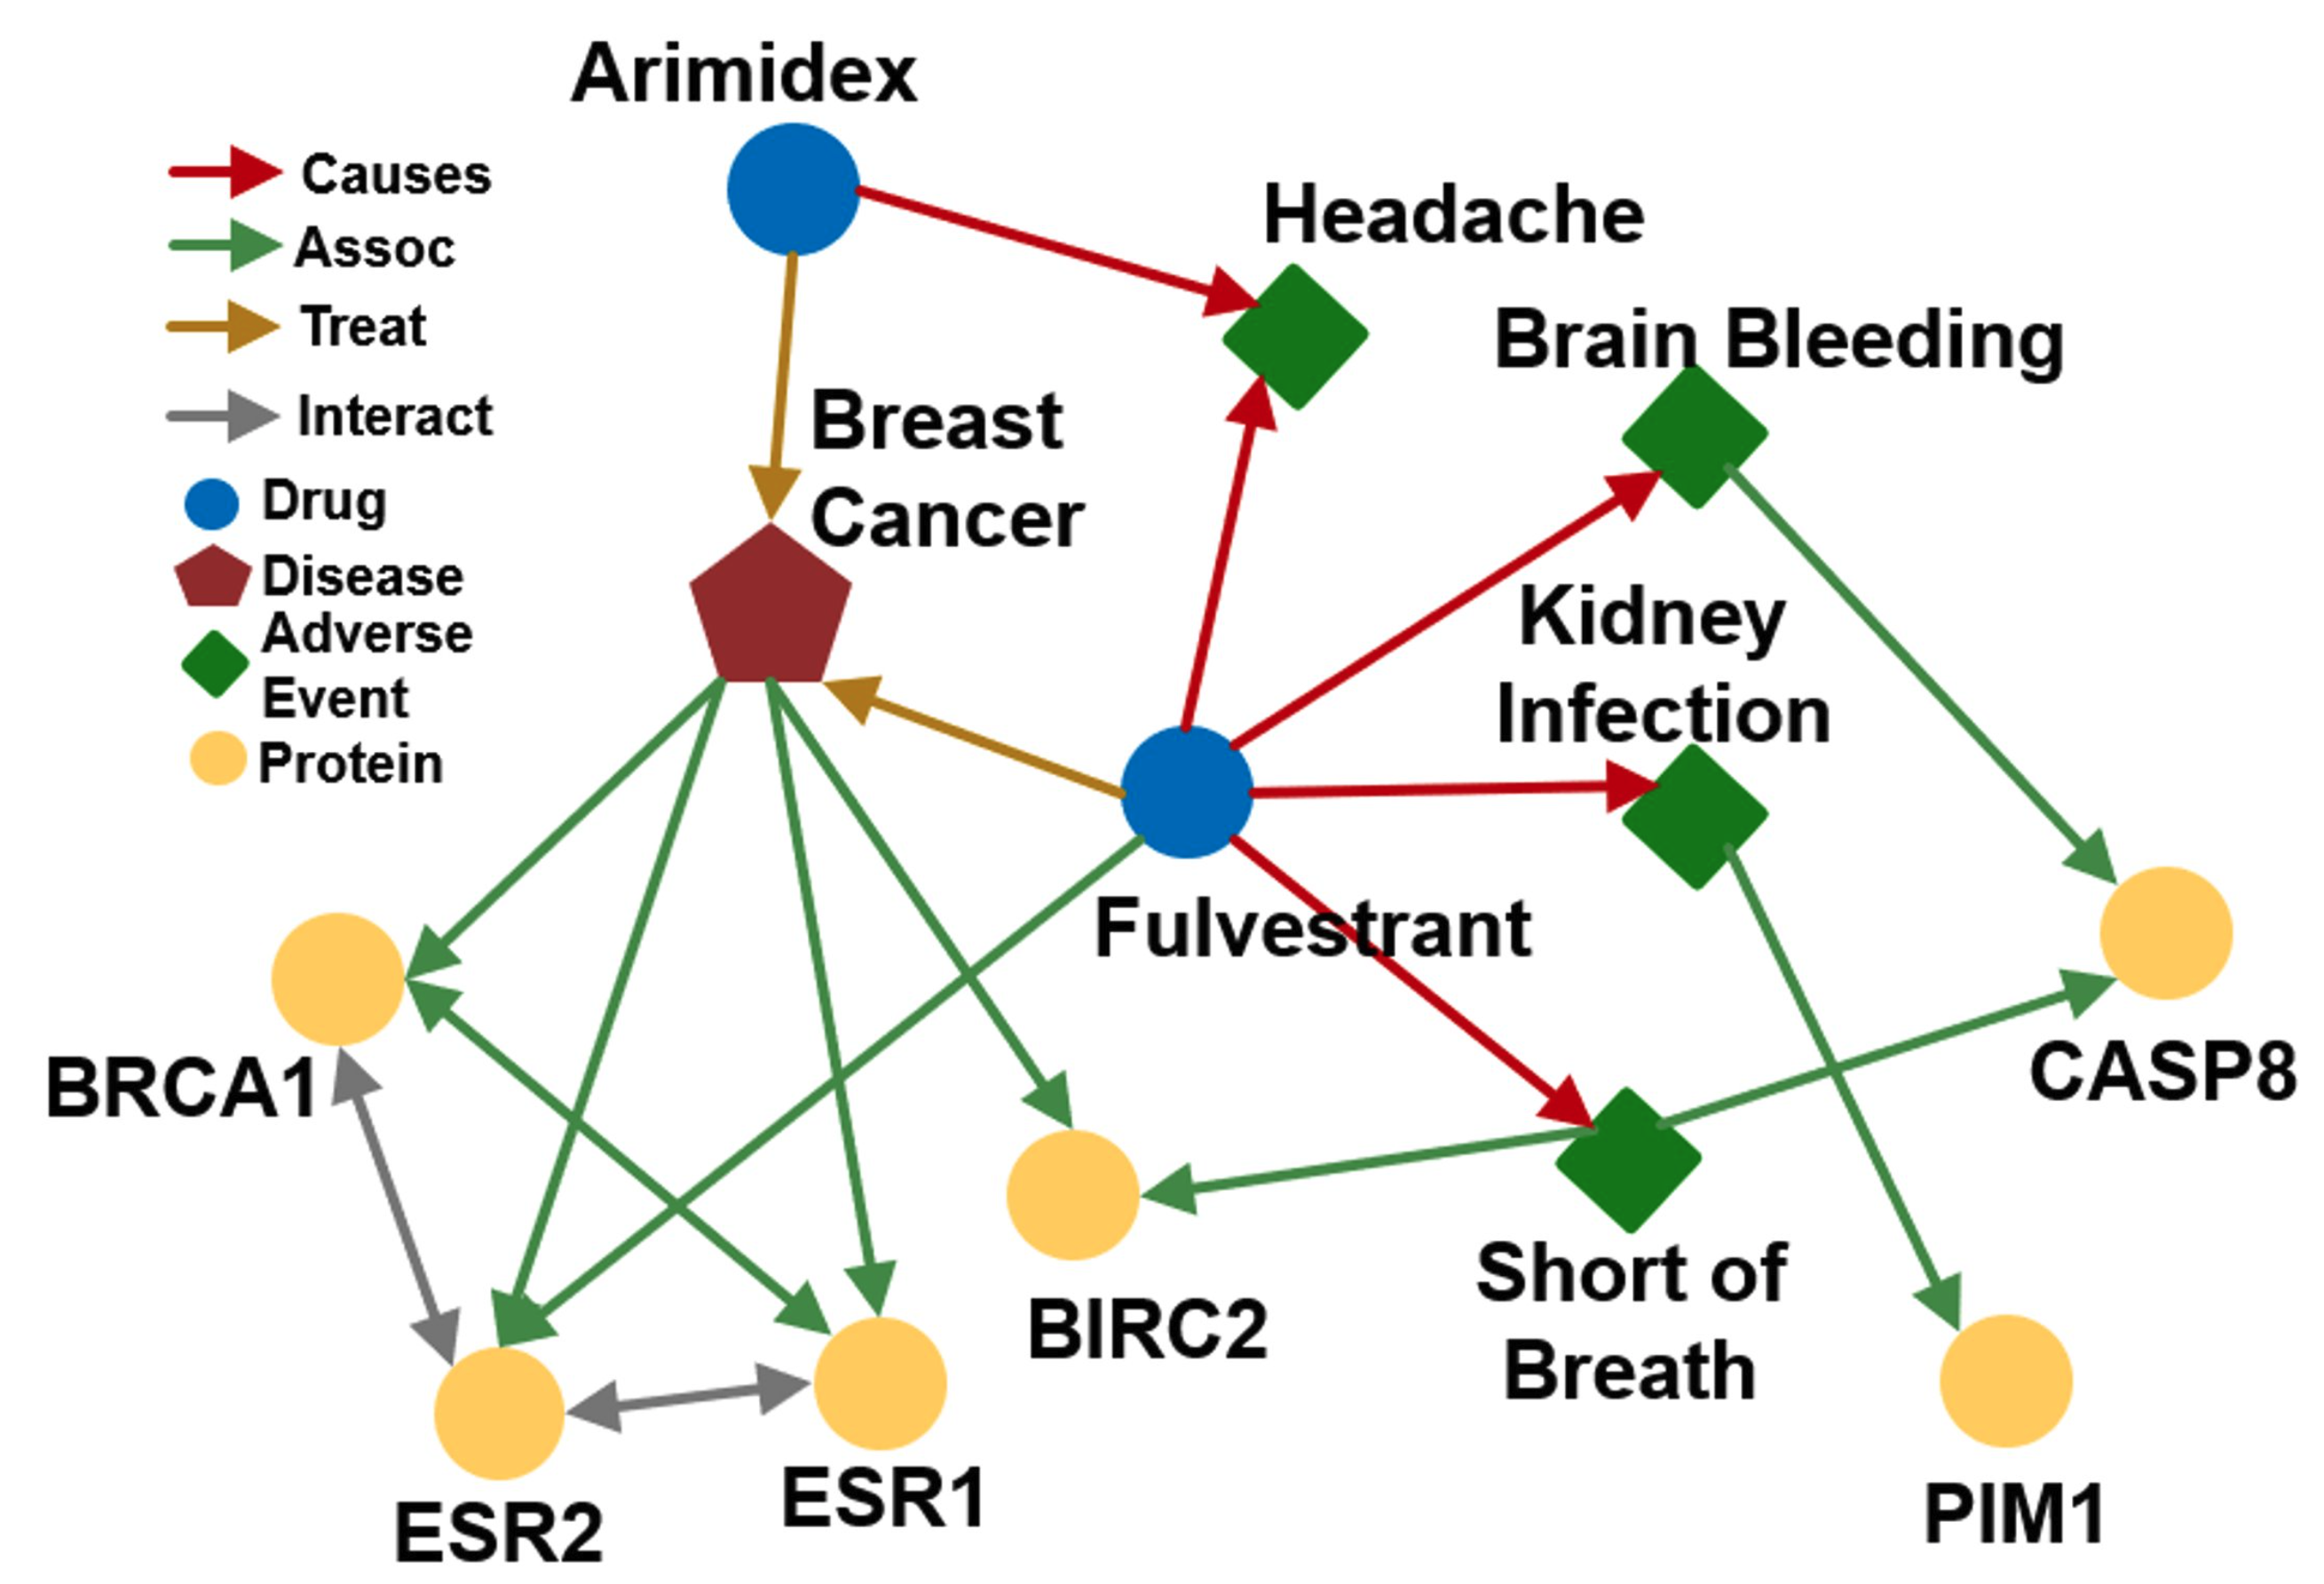
\includegraphics[width=0.8\textwidth]{5.1.png}
    \label{fig:5.1}
\end{figure}

\Solution{
	\textbf{Query Form:}
	The question "What proteins are associated with diseases treated by Arimidex?" can be broken down into a path query. We start at the anchor entity "Arimidex", find what it treats, and then find what proteins are associated with that disease.
	
	\begin{itemize}
		\item Anchor Entity (e): \texttt{Arimidex}
		\item First Relation (r1): \texttt{Treat}
		\item Second Relation (r2): \texttt{Assoc}
	\end{itemize}
	
	The query in the specified form is: \textbf{(e: Arimidex, (r: Treat, r: Assoc))}
	
	\textbf{Answer(s) to the Query:}
	To find the answers, we trace the path on the knowledge graph:
	\begin{enumerate}
		\item \textbf{Step 1:} Start at the anchor node \texttt{Arimidex}. Following the \texttt{Treat} edge (orange arrow) leads to the intermediate entity \texttt{Breast Cancer}.
		\item \textbf{Step 2:} From the intermediate node \texttt{Breast Cancer}, we follow all outgoing \texttt{Assoc} edges (green arrows) to find the final answer set. These edges point to three protein nodes.
	\end{enumerate}
	
	The final set of answers to the query is: \textbf{\{BRCA1, ESR1, BIRC2\}}
}


\subsection{Conjunctive Queries on Complete KGs [1 point]}
Consider the same biomedicine knowledge graph from before. Write a conjunctive query to which BIRC2 is the only answer using drugs as anchor entities. If such a query doesn't exist, provide a one-sentence explanation.

\Solution{
	No, such a query does not exist. Any path query starting from a drug anchor entity that reaches BIRC2 must first pass through Breast Cancer, and from Breast Cancer, the 'Assoc' relation also leads to BRCA1 and ESR1, making it impossible to isolate BIRC2 as the sole answer.
}


\subsection{Incomplete KGs [2 points]}
A major issue with direct traversals on knowledge graphs is that they are usually incomplete in reality. One solution is to encode entities, relations, and queries in an embedding space that meaningfully organizes information. We would then be able to impute missing relation links by considering all nearby points of the query embedding as answers to the query. From lecture, we learned that TransE embeddings can be used for this. Can you come up with a way to adopt DistMult embeddings, which uses bilinear modeling, for answering path queries? If yes, describe in one or two sentences what can be modified from the TransE application. If no, provide a one-sentence explanation.

\Solution{
	No, DistMult embeddings cannot be adapted to answer path queries in the same way as TransE. The core operation in TransE is vector addition, which allows a path query to be represented as a single query embedding by summing the anchor and relation vectors; however, DistMult's element-wise product operation does not have a similar mechanism for composing relations to represent a multi-hop path.
}


\subsection{Query2box [8 points]}

Query2box is an effective approach for answering complex conjunctive queries. Consider the following 2-dimensional embedding space. Assume that there are 7 entities $A, B, C, D, E, F, G \in V$, whose embeddings are shown below. There are 3 relations: $R_1, R_2, R_3$. $R_1 \in R$ shifts the center of a box by $(0.25, 2)$ and increases the width and height of a box by $(0.5, 2)$. $R_2$ shifts the center of a box by $(1, 0)$ and increases the width and height of a box by $(1, 0)$. $R_3$ shifts the center of a box by $(-0.75, 1)$ and increases the width and height of a box by $(1.5, 3)$.

Use the Query2box projection operator to find the answers to the conjunctive query: ((e:$A$, (r:$R_1$, r:$R_2$), (e:$C$, (r:$R_3$)). Show your work. Partial credit will be rewarded to correct intermediate steps.

Note: Shifting by a negative value means moving towards the left or bottom. Increasing the width and height by an amount means adding that amount in absolute value, not multiplying that amount as a factor. Assume that each path query starts with a box centered at the anchor entity with zero width and height.

\begin{figure}[H]
    \centering
    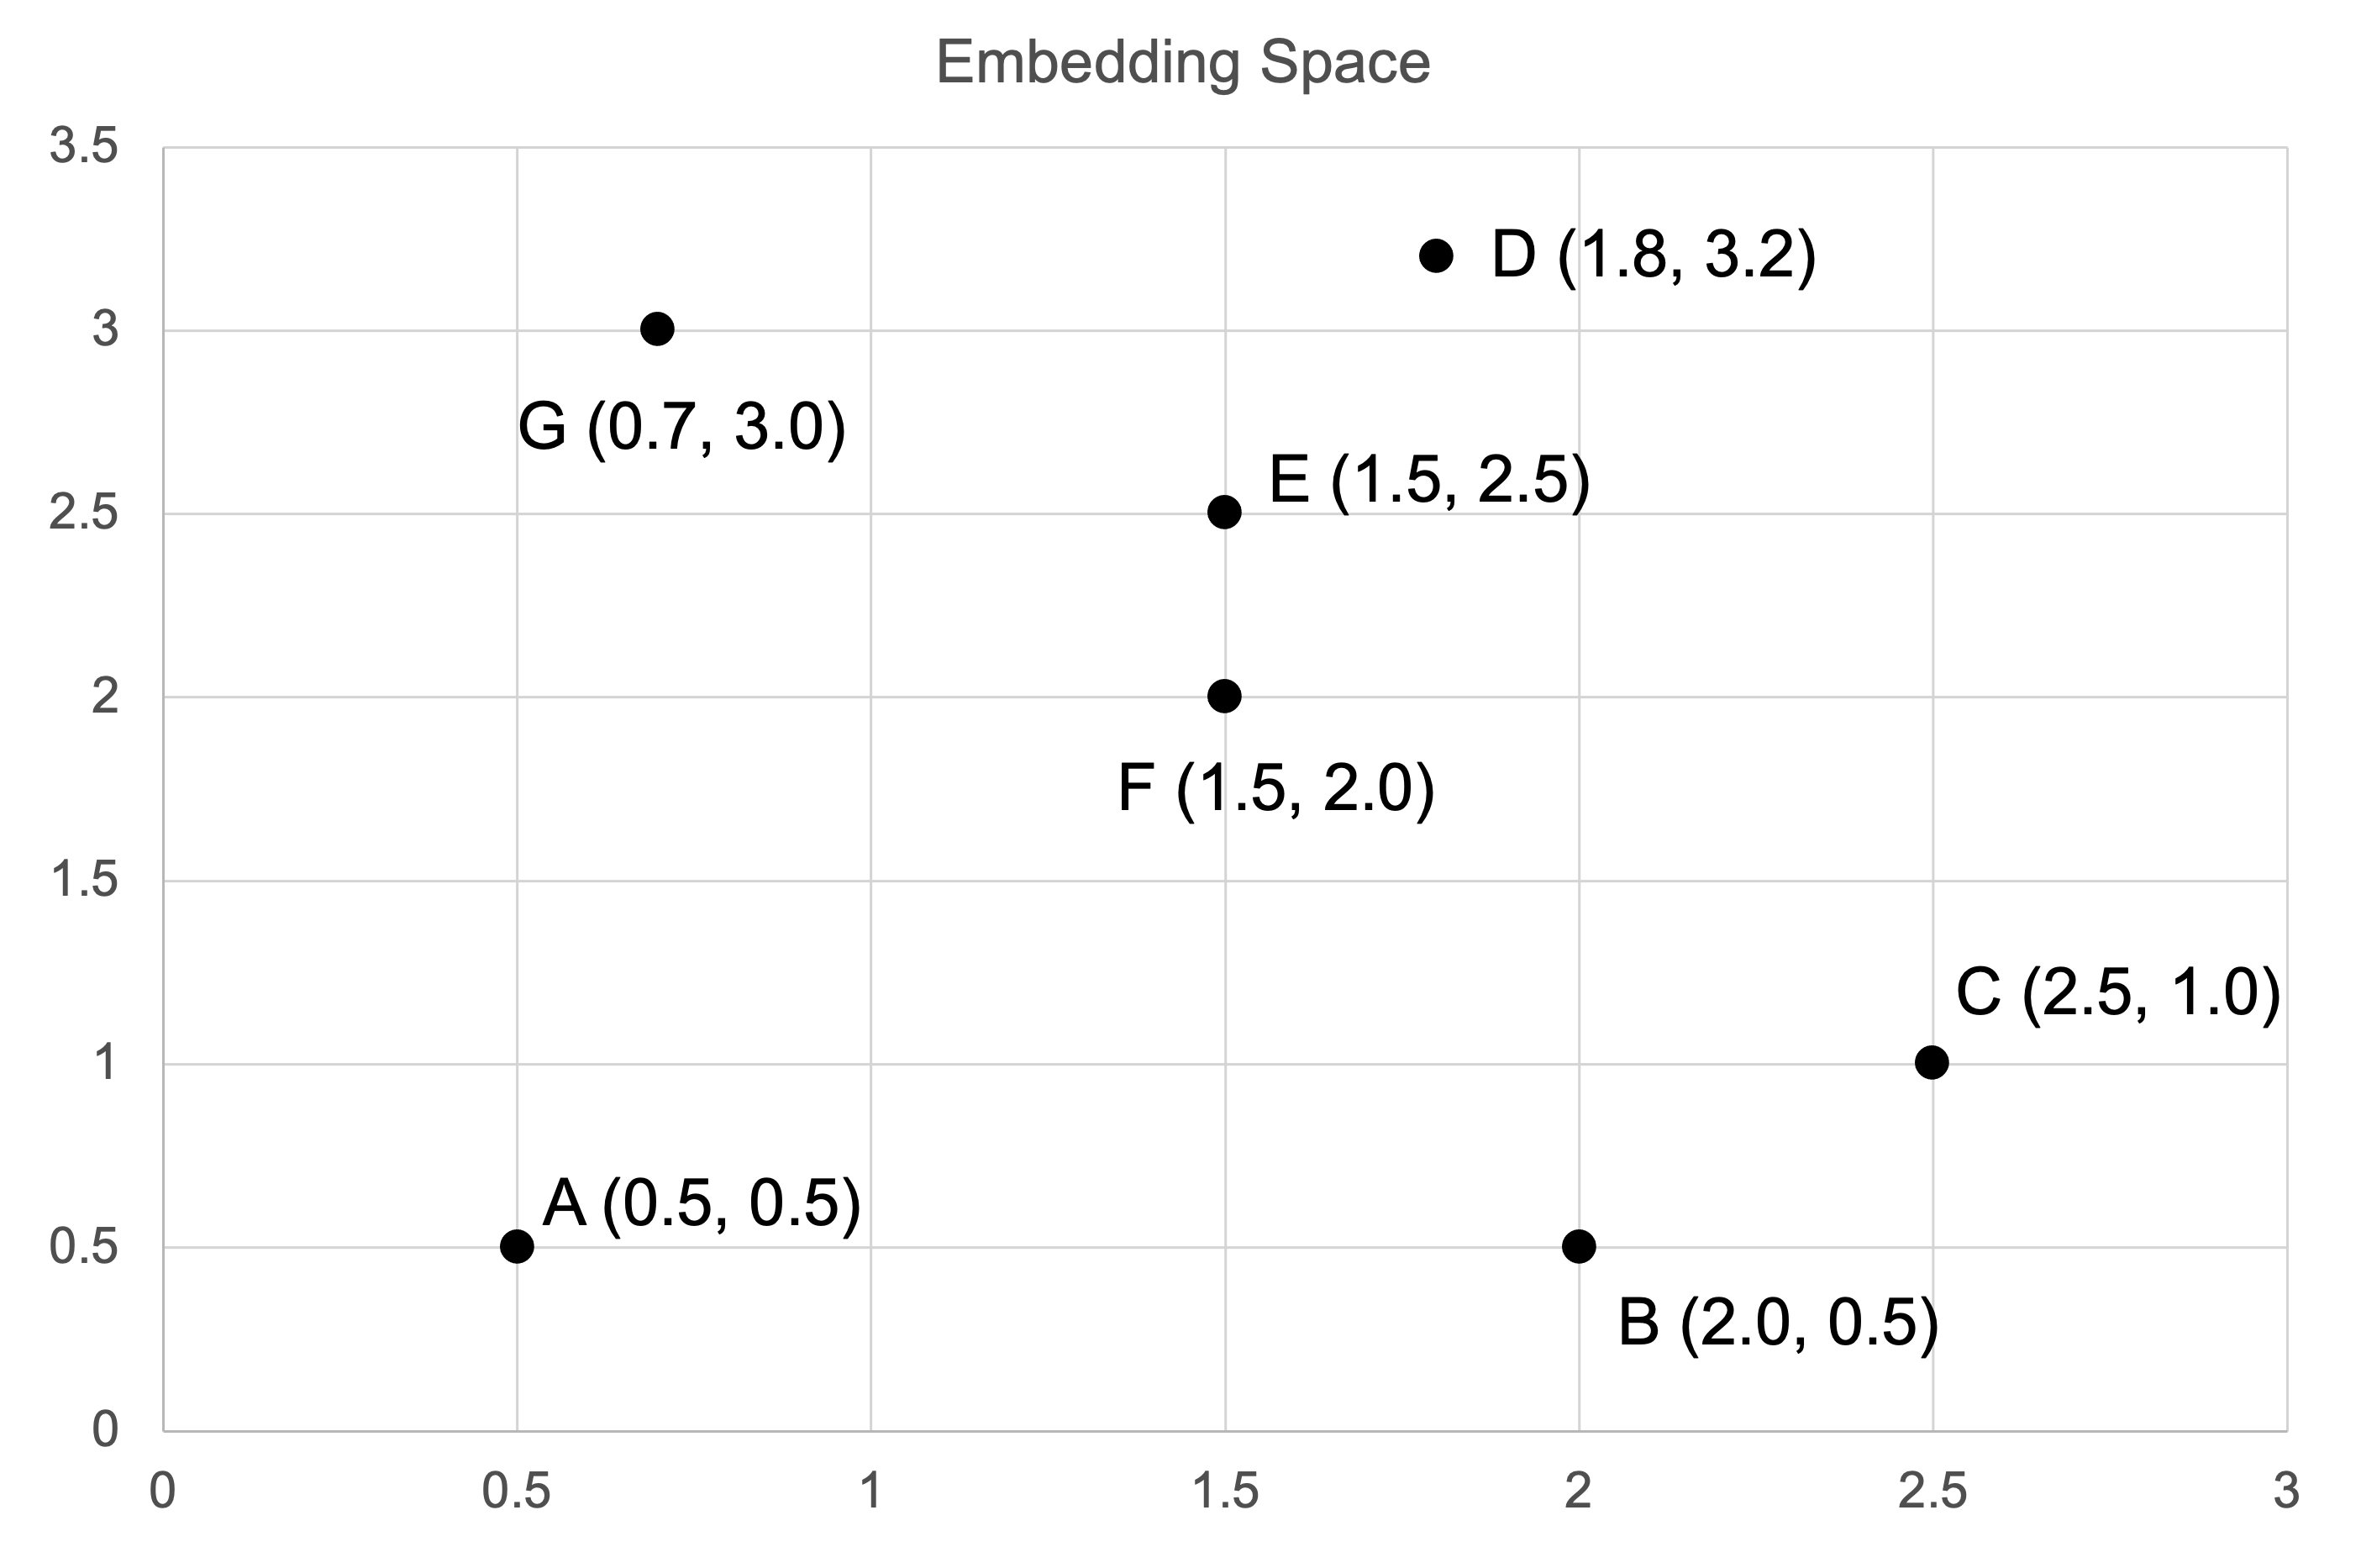
\includegraphics[width=0.9\textwidth]{5.4.png}
    \label{fig:5.4}
\end{figure}

\Solution{
	The final answer is the set of entities that lie within the intersection of the result boxes from the two path queries. We will solve each path query separately and then find the intersection of their answer sets.
	
	\textbf{Path Query 1: ((e:A, (r:R1, r:R2)))}
	\begin{enumerate}
		\item Start with a zero-sized box at anchor entity A:
		\begin{itemize}
			\item Center: (0.5, 0.5)
			\item Size (width, height): (0, 0)
		\end{itemize}
		\item Apply the projection for relation R1 (Shift by (0.25, 2), Increase size by (0.5, 2)):
		\begin{itemize}
			\item New Center: (0.5, 0.5) + (0.25, 2) = (0.75, 2.5)
			\item New Size: (0, 0) + (0.5, 2) = (0.5, 2)
		\end{itemize}
		\item Apply the projection for relation R2 (Shift by (1, 0), Increase size by (1, 0)):
		\begin{itemize}
			\item Final Center: (0.75, 2.5) + (1, 0) = (1.75, 2.5)
			\item Final Size: (0.5, 2) + (1, 0) = (1.5, 2)
		\end{itemize}
		\item Determine the boundaries of the final box for Query 1:
		\begin{itemize}
			\item X-range: $[1.75 - 1.5/2, 1.75 + 1.5/2] = [1.0, 2.5]$
			\item Y-range: $[2.5 - 2/2, 2.5 + 2/2] = [1.5, 3.5]$
		\end{itemize}
		\item The entities inside this box are: \textbf{\{D, E, F\}}.
	\end{enumerate}
	
	\textbf{Path Query 2: (e:C, (r:R3))}
	\begin{enumerate}
		\item Start with a zero-sized box at anchor entity C:
		\begin{itemize}
			\item Center: (2.5, 1.0)
			\item Size: (0, 0)
		\end{itemize}
		\item Apply the projection for relation R3 (Shift by (-0.75, 1), Increase size by (1.5, 3)):
		\begin{itemize}
			\item Final Center: (2.5, 1.0) + (-0.75, 1) = (1.75, 2.0)
			\item Final Size: (0, 0) + (1.5, 3) = (1.5, 3)
		\end{itemize}
		\item Determine the boundaries of the final box for Query 2:
		\begin{itemize}
			\item X-range: $[1.75 - 1.5/2, 1.75 + 1.5/2] = [1.0, 2.5]$
			\item Y-range: $[2.0 - 3/2, 2.0 + 3/2] = [0.5, 3.5]$
		\end{itemize}
		\item The entities inside this box are: \textbf{\{B, C, D, E, F\}}.
	\end{enumerate}
	
	\textbf{Final Answer (Intersection):}
	The answer to the conjunctive query is the intersection of the two answer sets:
	\[ \{D, E, F\} \cap \{B, C, D, E, F\} = \textbf{\{D, E, F\}} \]
}


% \input{Homework 2/problems/subgraph-order-embeddings}

\section{Honor Code [0 points]}
(X) I have read and understood Stanford Honor Code before I submitted my
work.

**Collaboration: Write down the names \& SUNetIDs of students you collaborated with on Homework 2 (None if you didn’t).**

**Note: Read our website on our policy about collaboration!**

\end{document}

